
% JuliaCon proceedings template
\documentclass{juliacon}
\setcounter{page}{1}

\usepackage{amsmath}
\usepackage[capitalise]{cleveref}
\crefname{equation}{}{}
\Crefname{equation}{}{}
\hypersetup{colorlinks}

\usepackage{tikz}
\usetikzlibrary{positioning, arrows.meta, fit, calc}

\begin{document}

% **************GENERATED FILE, DO NOT EDIT**************

\title{FMIExchange.jl: Foreign Models Through a Familiar Interface}

\author[1, 2]{Lucas Bex}
\author[1, 2]{Geert Deconinck}
\affil[1]{dept. of Electrical Engineering - KU Leuven}
\affil[2]{EnergyVille}

\keywords{Julia, Differential equation, Functional Mock-up Interface, Simulation}

\hypersetup{
pdftitle = {FMIExchange.jl: Foreign Models Through a Familiar Interface},
pdfsubject = {JuliaCon 2022 Proceedings},
pdfauthor = {Lucas Bex, Geert Deconinck},
pdfkeywords = {Julia, Differential equation, Functional Mock-up Interface, Simulation},
}



\maketitle

\begin{abstract}
The Functional Mock-up Interface (FMI) standard \cite{modelicaassociation} facilitates interoperability of differential algebraic equation (DAE) simulation software.
Compliant models (so-called Functional Mock-up Units (FMUs)) can be simulated through a standardized interface, which allows to easily exchange these models between different software tools.
The Julia ecosystem contains an extensive FMI package suite that supports (among others) simulation, import, export and differentiation of FMUs.
This paper presents FMIExchange.jl, which provides utilities to simplify interfacing FMUs with the popular DifferentialEquations.jl package \cite{rackauckas2017}.
Additionally, FMIExchange.jl provides tools to compose simulations combining multiple FMUs and native Julia models.
\end{abstract}

\section{Statement of Need}
The Functional Mock-up Interface (FMI) standard \cite{modelicaassociation} presents a standardised software interface for simulating an ordinary differential equation (ODE) with events to enhance interoperability of simulation and modelling tools.
Many differential algebraic equation (DAE) modelling tools have the possibility to export models (after transformation to an ODE) to Functional Mock-Up Units (FMU, \cref{fig:FMU}), which comply with this interface.

FMUs define a set of states states $u$ and inputs $p_i$ required for simulating the model \cref{eq:ODE}, as well as a set of outputs $p_o$ \cref{eq:output} which are exposed to the user.
FMUs may contain events, that cause discontinuouties in the solution of the ODE.
Events may trigger at fixed times or whenever the state/inputs fulfil some condition.
Three types of FMU are available: Co-Simulation FMUs only expose inputs and outputs and come bundled with an integrator and event handler, Model Exchange (ME-)FMUs require an external ODE integrator/event handler and expose all quantities, Scheduled Execution FMUs expose model partitions, algorithms to compute quantities of interest, and require a scheduler to trigger execution of these model partitions; this text focuses on ME-FMUs.
\begin{align}
f(u, p_{i}, t) &= \dot{u} \label{eq:ODE}\\
g(u, p_{i}, t) &= p_o \label{eq:output}
\end{align}

\begin{figure}
  \center
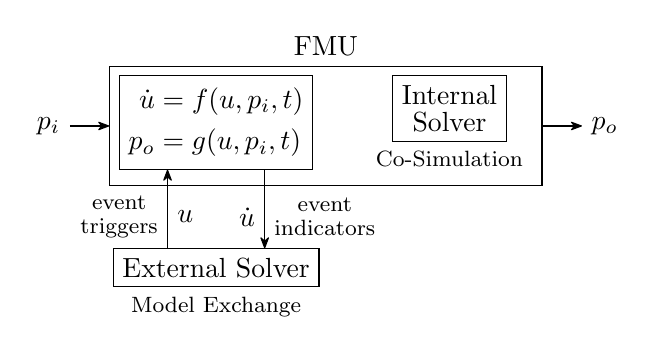
\begin{tikzpicture}[node distance=0.5cm, >={Stealth[round]}]
  \node (FMUeq) [draw=black] {$\begin{aligned}
    \dot{u} &= f(u, p_{i}, t) \\
    p_o &= g(u, p_i, t)
  \end{aligned}$};
\node (CS) [right=1cm of FMUeq.north east, anchor = north west, draw=black, label={[name=CSL]below:\footnotesize Co-Simulation}] {\shortstack{Internal\\Solver}};
  \node (FMU) [draw=black, label=above:FMU, minimum width=5cm, fit=(FMUeq) (CS) (CSL)] {};
\node (u) [left=of FMU] {$p_i$} edge [->] (FMU);
\node (y) [right=of FMU] {$p_o$} edge [<-] (FMU);
% \node (xdot) [below=of FMU, xshift=0.75cm] {$\dot{u}$} edge [<-] (FMU.south -| xdot);
% \node (x) [below=of FMU, xshift=-0.75cm] {$u$} edge [->] (FMU.south -| x);
\node (ME) [below=1cm of FMUeq, draw=black, label={[name=MEL]below:\footnotesize Model Exchange}] {External Solver};
\coordinate (e1) at ($(FMUeq.south east)!0.5!(FMUeq.south)$ |- ME.north);
\coordinate (e2) at ($(FMUeq.south west)!0.5!(FMUeq.south)$ |- ME.north);
\draw [->] (e1) -- node [auto, swap, yshift=-1mm] {$\dot{u}$} node [auto, yshift=-1mm] {\footnotesize \shortstack{event\\indicators}} ($(ME.north west)!(e1)!(ME.north east)$);
\draw [<-] (e2) -- node [auto, yshift=-1mm] {$u$} node [auto, swap, yshift=-1mm] {\footnotesize \shortstack{event\\triggers}} ($(ME.north west)!(e2)!(ME.north east)$);
% \draw[->] (FMU.south -| ME) -| node [near end, auto] {$\dot{u}$} node [near end, auto, swap] {\footnotesize \shortstack{event\\indicators}} (solver.north -| ME);
% \draw[->] (solver.north -| ME) -| node [near end, auto, swap] {$u$} node [near end, auto] {\footnotesize \shortstack{event\\triggers}} (FMU.south -| ME);
\end{tikzpicture}
\caption{FMUs present a standardized software interface for simulating ODEs. A solver can be bundled with the FMU (Co-Simulation) or the FMU may use an external solver (Model Exchange).}
\label{fig:FMU}
\end{figure}

An FMU bundles an ODE model into a (binary) shared library and accompanying XML description of the model; this allows to call the model from other programs e.g. using Julia's \texttt{ccall} functionality.
Within the Julia ecosystem, FMI.jl and related packages \cite{thummerer2021} provide powerful functionality for interacting with and simulating individual FMUs.
While it is possible to combine FMUs with other (native Julia or FMU-based) models using aforementioned packages, this requires familiarity with the FMI standard and significant effort from the user to ensure correctness.
FMIExchange.jl aims to simplify this process and make FMUs easier to use for an audience that is unfamiliar with the FMI standard.
To this end, FMIExchange.jl predefines callbacks to correctly handle FMU events and integration.
Additionally, some functionality is provided to simplify composing multiple (FMU-based or native) models in a single DifferentialEquations.jl-based simulation.

\section{Composition Functionality}
\label{sec:composition}
To compose multiple models in a simulation, their inputs/outputs must be appropriately connected to each other and all dynamics must be bundled into a single function of the form \texttt{f(u, p, t)} or \texttt{f!(du, u, p, t)} and a set of callbacks.
To this end, FMIExchange.jl works with the simulation model depicted in \cref{fig:simulation}: all model states $u_j$ are bundled in a flat \texttt{u} vector; model inputs/outputs are connected through an intermediate buffer which is the parameter \texttt{p} argument in \texttt{f}.
The \texttt{p} argument is accessible both to callbacks and the dynamics functions and thus this approach allows for the most flexibility in composing simulations.
Here, FMIExchange.jl differs from other packages, such as most packages in the SciML ecosystem, because the \texttt{p} argument is used to store time-varying quantities rather than parameters which are fixed during the simulation.

To aid the user in composing simulations of the format in \cref{fig:simulation}, FMIExchange.jl provides i) functionality to combine dynamics functions $f_j$ into a DifferentialEquations.jl-compatible function \texttt{f} (with in-place and out-of-place methods), ii) predefined callbacks to automatically update model output between integration timesteps, and iii) human-readable address map generation functionality for both the \texttt{u} and \texttt{p} argument.
FMIExchange.jl does not provide any simulation capabilities itself; it merely generates callbacks and dynamics functions to use in the DifferentialEquations.jl framework.
In this manner, the user retains the full flexibility of the DifferentialEquations.jl interface: it is possible to use the capabilities of FMIExchange.jl to compose some models, and bypass it for other models in that same simulation.
This flexibility includes the ability to reintroduce fixed simulation parameters back into the \texttt{p} vector if so desired.

\begin{figure}
  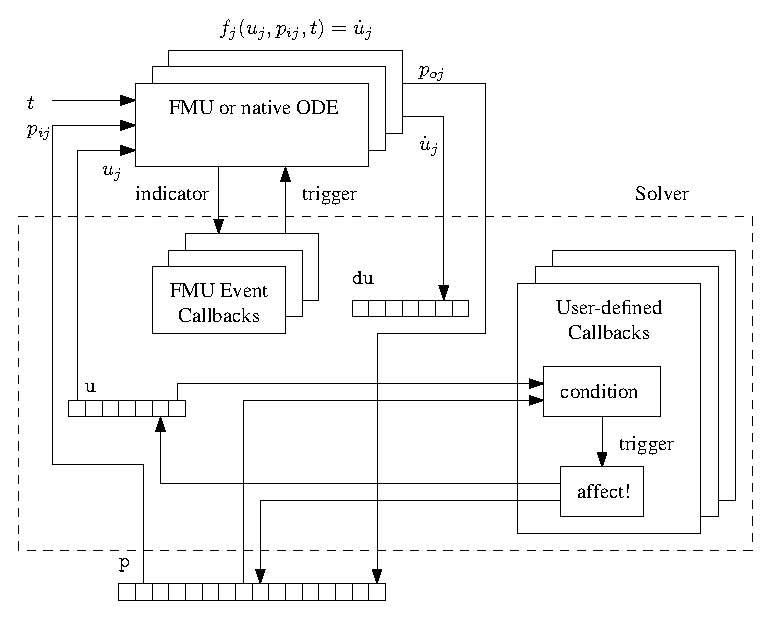
\includegraphics[width=\columnwidth]{graphics/simulation.eps}
  \caption{Composing multiple models in a simulation}
  \label{fig:simulation}
\end{figure}

For the addressing and state/input/output bundling functionality, FMIExchange.jl relies on custom types \texttt{AbstractSimModel} and \texttt{AbstractModelSpecification}.
Addresses in the form of indices of \texttt{p}/\texttt{u} and model functionality (dynamics function and callbacks) are contained in the \texttt{AbstractSimModel}.
The \texttt{AbstractSimModel} (or a vector of them) is used when bundling the dynamics functions and generating callbacks for automatically calling model output functions between integration steps.
To avoid having to manually assign addresses and provide a human-friendly interface, FMIExchange.jl can automatically generate address maps from human-readable \texttt{AbstractModelSpecification}s.
\texttt{AbstractModelSpecification}s specify states/inputs/outputs by name rather than address and can be converted directly into \texttt{AbstractSimModel}s using an address map.
For a practical example of a workflow, consult \cite{bex2024}.

\section{FMU Utilities}
Function Mock-Up Units are merely a special kind of model to include in a simulation.
As such, all functionality from \cref{sec:composition} is the same for native ODE models and ME-FMU models.
However, if not using FMIExchange.jl, correctly handling integration of ME-FMUs requires the user to interact directly with the FMU code object as implemented by the FMI.jl package which adheres strictly to the FMI standard.
FMIExchange.jl handles this for the user and does not require any familiarity with FMI.jl or the FMI standard.
Note that it is possible to simulate multiple FMUs and native ODEs using solely FMI.jl and DifferentialEquations.jl, but FMIExchange.jl greatly simplifies this process through its \texttt{AbstractSimModel} interface.
The FMU-handling functionality can be used on its own or together with the simulation composition functionality in \cref{sec:composition}.

FMIExchange.jl exposes all FMU states/inputs/outputs in the \texttt{u} and \texttt{p} variables for easy access.
Additionally, FMIExchange.jl can generate dynamics functions and callbacks that correctly embed the FMU in a DifferentialEquations.jl simulation.
The functionality includes: handling time-based, state-based and input-based FMU events, switching between FMU modes for calculating derivatives/calculating events/finishing integration steps, and automatically recalculating FMU outputs after an integration step.
Finally, FMIExchange.jl implements the \texttt{CachedModel} struct which preallocates caches to avoid excessive memory allocations at each \texttt{ccall} call to the FMU.

FMIExchange.jl is currently only compatible with FMI version 2 \cite{modelicaassociation2022}.

\section{Conclusion}
FMIExchange.jl simplifies composing complex simulations with multiple interacting ODE models that are implemented either in Julia or as a Functional Mock-up Unit.
The package achieves this by providing functionality for bundling model dynamics functions of different models and for easily generating various commonly needed callbacks to embed in a DifferentialEquations.jl simulation.
Automatic address map generation and support for human-readable addresses is included in the package to simplify composition of many models in a simulation.
FMIExchange.jl itself does not provide any simulation functionality, but allows the user to retain full control through the powerful DifferentialEquations.jl interface.

Within this framework, Functional Mock-up Units are merely another type of model, allowing seamless composition of native Julia and FMU-based models.
FMIExchange.jl provides functionality for automatically generating the required callbacks and dynamics function for correct FMU simulation.
As a result, users can easily compose native Julia models and FMUs in a single simulation, without requiring extensive knowledge of the FMI standard.

\section{Acknowledgements}
The authors acknowledge the financial support from KU Leuven through the TECHPED - C2 project (C24M/21/021) and the Research Foundation - Flanders (FWO) (grant no. 1S00325N).

\input{bib.tex}

\end{document}

% Inspired by the International Journal of Computer Applications template
